\section{Solution Architecture}
\label{sec:solution_architecture}
% -----------------------------------------------
% STATE OF ART
% -----------------------------------------------
\subsection{State of the Art}
\label{sub:state_of_art}
Cloud-based IoT applications are the state-of-the-art of this kind of solutions. By leveraging
the infrastructure to the Cloud providers, these applications have a high-availabity, can dynamically
scale while spending a fraction compared with the traditional solutions. However, as earlier
mentioned the deployment of such applications still is an issue, due its complexity and
required manual intervention. The deployment of Cloud-based IoT applications usually are performed
through IT automation tools, such as Chef\footnote{http://www.chef.io} and Puppet\footnote{http://www.puppetlabs.com}.
These automate the deployment of applications. However, the components of the application and the relation between
themselves must be specified manually, which requires considerable manual work and expertise by the person that
is performing the deployment. The deployment process of these solutions is not the only existing issue.
Monitoring the application life-cycle is a task that requires a lot of effort and expertise by the system
administrators.\\

In order to solve this problem, the adopted approach relies on using Cloud Orchestrator tools perform the
deployment of these applications. As mentioned in \textbf{\ref{subs:cloud_orchestration}},
these tools allows the specification of the application components and their relations in a high-level perspective
and to execute the management tasks required by the application during its life-cycle. As a matter of fact,
in a low-level perspective cloud orchestration tools express the high-level perspective defined by the user
into scripts that latter are executed using IT automation tools such as Puppet and Chef.
% -----------------------------------------------
% CLOUD4THINGS ARCHITECTURE
% -----------------------------------------------
\subsection{Cloud4Things Architecture}
\label{sub:cloud4things_architecture}
The architecture of Cloud4Things is based in the perspectives that are
used to describe an information system according the Zachman framework \cite{}.
In this framework Zachman defines the \textit{Conceptual}, \textit{Logical} and
\textit{Technological} perspectives that allows to describe an information system
from a more abstract to a more detailed view.
% ----------------------------------------------
% CONCEPTUAL ARCHITECTURE
% ----------------------------------------------
\subsubsection{Conceptual Architecture}
\label{subs:conceptual_architecture}
The \textit{Conceptual} architecture describe Cloud4Things in perspective of
the business entities and processes that compose the system and how they are related,
as illustrated in Figure~\ref{fig:conceptual_architecture}.
% Cloud4Things conceptual architecture
\begin{figure}[h!]
  \centering
  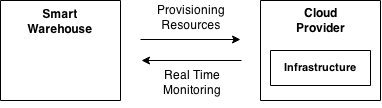
\includegraphics[width=.8\textwidth]{./images/conceptual-architecture}
  \caption{Cloud4Things Conceptual architecture.}
  \label{fig:conceptual_architecture}
\end{figure}\\
The business entities that composes Cloud4Things are the smart smart place and the
Cloud provider. The smart place uses an Internet connection to access the resources
that are allocated in the Cloud infrastructure. The Cloud providers allow the smart
places to perform real-time monitoring of the used resources.
% ----------------------------------------------
% LOGICAL ARCHITECTURE
% ----------------------------------------------
\subsubsection{Logical Architecture}
\label{subs:logical_architecture}
The \textit{Logical} architecture describe Cloud4Things in perspective of
the data elements, logical process flows and functions that represent business
entities and processes, as illustrated in Figure~\ref{fig:logical-architecture}.
% Cloud4Things logical architecture
\begin{figure}[h!]
  \centering
  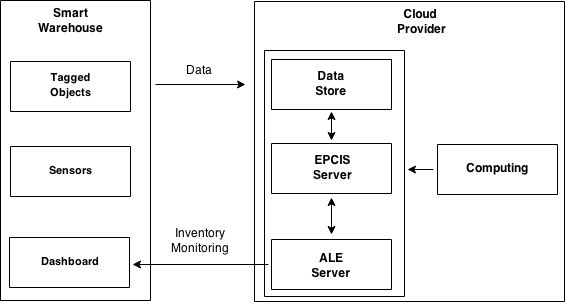
\includegraphics[width=.8\textwidth]{./images/logical-architecture}
  \caption{Cloud4Things Logical architecture.}
  \label{fig:logical_architecture}
  \end{figure}\\
% ----------------------------------------------
% TECHNOLOGICAL ARCHITECTURE
% ----------------------------------------------
\subsubsection{Technological Architecture}
\label{subs:technological_architecture}
% ----------------------------------------------
% MONITOR AGENT ARCHITECTURE
% ----------------------------------------------
\subsubsection{Monitor Agent Architecture}
\label{subs:monitoring_srchitecture}
\vspace{1in}
% Cloud of Things Architecture
\begin{figure}[h!]
  \centering
  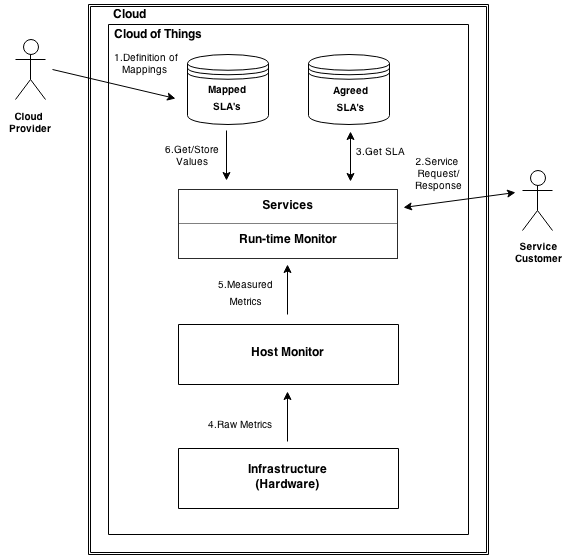
\includegraphics[width=.8\textwidth]{./images/cloud-of-things-architecture}
  \caption{Cloud of Things Architecture.}
  \label{fig:cloud_of_things_architecture}
\end{figure}
The presented architecture is based on the LoM2HiS Framework \cite{emeakaroha2010low} architecture. The
\textit{Host Monitor} processes the monitored values of the hardware and network resources that are delivered
by monitoring agents that are embedded in the infrastructure. The \textit{Run-time Monitor} is responsible to
monitor the customer application (\textit{Services}) status and performance based on the negotiated
and agreed SLAs.\\

The monitoring process starts after the Cloud provider agrees on the SLA terms.
The agreed SLAs are stored in the repository for service provisioning and the following
steps are executed:
\begin{enumerate}
  \item The Cloud provider creates rules for the framework mappings of low-level metrics (QoS parameters) using Domain Specific
  Languages\footnote{Domain Specific Languages are small languages that normally are tailored to a specific
  problem domain.} (DSLs).
  \item The customer requests the provisioning of an agreed service.
  \item Once the request is received, the run-time monitor loads the service SLA from the agreed SLA repository.
  \item The resource metrics are measured by monitoring agents, these metrics are stored in a raw format that
  later are accessed by the host monitor.
  \item The host monitor extracts metric-value pairs from the raw metrics and them transmits them periodically to
  the run-time monitor.
  \item After receiving the low-level metrics, the run-time monitor uses predefined mapping rules to map the
  low-level metrics into an equivalent form of the agreed SLA and them the resulting map is stored in the
  mapped metrics repository.
\end{enumerate}

In this architecture, the \textit{Run-time monitor} uses the mapped values to monitor the status of the deployed services.
Once it detects that a SLA is violated, the \textit{Run-time monitor} must alert the customer of the violated SLA.
